\chapter{Discussion}

In this Chapter I will discuss how my results fit into the `big picture' of galaxy evolution and discuss their broader implications (Section~\ref{sec:bigpic}). I will then discuss future work with \starpy\ (Section~\ref{sec:future}) and how I intend to adapt it so that it can be applied to IFU spectral data (Section~\ref{sec:IFU}). I will then end with a reflection on the power of Hubble Space Telescope imaging in comparison to SDSS imaging. 

%I will also discuss the implications my results have for the proper use of morphology in galaxy evolution studies (Section~\ref{sec:usemorph}).

\section{The Big Picture}\label{sec:bigpic}

In this thesis I have investigated quenching as a function of colour, morphology, the presence of an AGN and environmental properties across a large galaxy population. I have found that the green valley is tracing the evolution of the red sequence and that though there is a morphological dependance on the rate that quenching will preferentially occur, galaxies of any morphology can quench at any rate (Chapter~\ref{chap:morph}). I have found that lower mass galaxies hosting an AGN have quenched rapidly and recently, suggesting that the AGN may be the direct cause of this quenching through feedback (Chapter~\ref{sec:agnfeedback}). However, I have also shown that quenching in AGN host galaxies does not always proceed rapidly, suggesting a slower co-evolution of galaxies with their black holes. I investigated this slower evolutionary history with a sample of assumed merger free bulgeless AGN host galaxies which were found to host black holes which were much more massive than predicted by typical black hole scaling relations (Chapter~\ref{intbulgeless}). I have also found evidence for environmentally driven quenching mechanisms, mass quenching and morphology quenching within the group environment; the derived timescales for which imply that environmentally driven quenching mechanisms must work in sync to quench a satellite galaxy (Chapter~\ref{chap:env}). I shall now discuss how all of these results fit into the `big picture' of galaxy evolution. 

In Chapter~\ref{chap:morph} I considered how my results suggested that quenching rates with $\tau < 1.5~\rm{Gyr}$ must be caused by mechanisms which can transform a galaxy from a disc to an elliptical. However this does not infer an immediate transition from a disc dominated to a bulge dominated galaxy. Work by the \textsc{ATLAS}$^{\rm{3D}}$ team \citep{cappellari11} showed in the majority of the visually elliptical population are rotationally supported \citep{emsellem11} with $\sim7$ times the number of \emph{fast rotators} (with kinematic discs) than \emph{slow rotators} \citep[with dispersion dominated kinematics see][]{cappellari07, emsellem07}.  This has led to the proposal of a revision of Hubble's morphological classification scheme in the form of a ``comb" \citep[see Figure 24 of the review paper by]{cappellari16}, whereby the evolution of a disc galaxy from disc to bulge dominated takes place along a tine of the comb, until they become bulge dominated fast rotators. These fast rotators then evolve along the handle of the comb to become slow rotators. Given the nature of the GZ classifications, both fast and slow rotators will most likely have been classified as smooth galaxies and so both are expected to contribute to the smooth weighted populations shown in Chapters~\ref{chap:morph} \& \ref{chap:agn}. We must therefore consider how this will impact the conclusions made in Chapter~\ref{chap:morph}. 

Dry major mergers are considered the most likely process to produce slow rotators \citep{duc11, naab14} as they can destroy the disc dominated nature of a galaxy \citep{toomre72} in rapid timescales. I find that across the red smooth weighted population in Figure~\ref{red_s} that $12\%$ of the population density lies below $\tau <0.2~\rm{Gyr}$, in agreement with predictions that between $14-17\pm5\%$ of ellipticals are slow rotators \citep{emsellem11, stott16}, suggesting that quenching mechanisms with these rates might give rise to a slow rotator. This therefore also provides an estimate for the percentage of the galaxy population which have undergone a dry major merger, estimated to be approximately $10-20\%$ \citep[since $z\sim1$;][]{khochfar09}.

Fast rotators are theorised to be formed by the slow build up of a galaxy's bulge over time, until it eventually overwhelms the disc. This growth is thought to occur via gas-rich major and minor mergers \citep{duc11} which can produce a bulge dominated, rotationally supported quenched galaxy, which would be visually classified as an elliptical. Although these mechanisms do not completely destroy the disc of a galaxy, they do cause an eventual morphological change to a bulge dominated galaxy. This could be the source of the result suggesting all mechanisms with $\tau < 1.5 ~\rm{Gyr}$ must be able to cause a morphological change during quenching in order for the ratio of smooth : disc galaxies in the green valley to match that of the red sequence. Although this morphological change does not produce a true dispersion dominated elliptical galaxy, the resultant galaxy will be identified as smooth by the GZ users. Despite this, the \textsc{popstarpy} method has still managed to reveal this important, slightly slower process of producing a bulge dominated galaxy and separate it from the rapid rates caused by dry major mergers (see Figures~\ref{red_s} \& \ref{green_v}). The larger IFU studies of MaNGA, SAMI and CALIFA will allow for larger populations of slow and fast rotators to be identified so that the relative dominance of gas-rich and dry mergers across the visually elliptical population can be determined more accurately (see Section~\ref{sec:IFU}). 

The rare \citep[$<1\%$;][]{Wong12, wild16} `missing link' post-starburst (PSB) galaxy phase is also thought to be linked with merger activity \citep{zabludoff96, blake04, goto05b, yang08, pawlik16}. PSBs are thought to have undergone an intense, unsustainable period of star formation in the recent past which has then rapidly quenched \citep{dressler83, abraham96b, poggianti99, goto03, goto05b, goto07} and can add a significant fraction \citep[$\sim10\%$;][]{wild10} to the stellar mass of a galaxy. \citet{Wild09}, who by making assumptions for how long galaxies spend in a PSB phase, estimated that gas rich major merger induced starbursts, which can simultaneously cause a morphological change, could account for $38\%$ of the growth of the red sequence at $z\sim0.7$. Figure~\ref{red_s} shows that $\sim40\%$ of the smooth weighted red population undergoes quenching at rates less than $0.7~\rm{Gyr}$, suggesting that these quenching rates could be associated with this post-starburst transition phase. 

However, earlier in this Section, I discussed how these quenching rates were also associated with the production of fast rotators. Work by \citep{pracy13} found that of the 26 `E+A' galaxies with kinematics 22 ($\sim85\%$) were classed as fast rotators. Although at first this result seems to suggest a connection between the PSB phase and fast rotator production, this fraction is in fact similar to the overall fraction of fast rotators found in the normal elliptical galaxy population \citep{emsellem11, stott16}. These kinematic studies of PSBs also allow the locations of the recent starbursts to be determined through spectral indicators of star formation \citep[such as $H\alpha$;][]{kennicutt94}. The recent distribution of the first data releases from MaNGA \citep[SDSS DR13;][]{albareti16}, SAMI \citep[EDR;][]{allen15} and CALIFA \citep[DR3;][]{sanchez16} will add to the known PSB galaxies which have be classified as either fast or slow rotators. Using \starpy\ to determine the spatially variant SFHs of these galaxies may help to further disentangle the theorised connection between PSBs and elliptical galaxies and the estimated contribution to the growth of the red sequence by this rare, short-lived, yet perhaps crucial evolutionary phase. 

Having now considered the effects of both major and minor mergers, let us turn our attention to an internal, secular quenching mechanism. A parameter which is often investigated in quenching studies is the stellar mass surface density of a galaxy, which is found to correlate with SFR \citep{barro13b, whitaker16}. As a galaxy's bulge grows it is thought to be able to stabilise a disc against collapse and effectively stop it from forming stars. This is classed as a type of morphological quenching and is effective over a few $\rm{Gyr}$ \citep{Fang13} even if external gas is still fed to a galaxy. This slower quenching track of bulge dominated galaxies may help to explain the slow quenching rates observed across the red and green smooth weighted population densities where slow quenching ($\tau>2~\rm{Gyr}$) of smooth galaxies is occurring in up to $40\%$ of the smooth weighted green population density (see Figure~\ref{green_v}) and $24\%$ of the smooth weighted red population (see Figure~\ref{red_s}). With \starpy\ this slower quenching history caused by processes which grow the bulge then consequently trigger morphological quenching has been separated out from more rapid quenching histories caused by processes which simultaneously quench and grow the bulge. 

However, even in the latter case, morphological quenching may help in either speeding up the quenching process or in ensuring the galaxy stays quenched. This is supported by the finding of \cite{abramson16} who found there is no threshold at which density triggered quenching occurs, but that denser systems typically redden faster than less dense galaxies. This suggests that minor mergers and morphological quenching work together to fully achieve quiescence, similar to the collaboration between starvation and stripping to achieve quiescence of satellite galaxies discussed in Chapter~\ref{chap:env}. 

A partnership between two quenching mechanisms was also discussed in Chapter~\ref{chap:morph}; simulations have shown that without AGN feedback a major merger cannot fully quench a galaxy \citep{springel05b}. Figure~\ref{rate} shows that galaxies in the \textsc{agn-host} population don't always quench at the rapid rates caused by major mergers, suggesting that a slow co-evolution of black hole and host galaxy can occur. Alone AGN are only an efficient quenching mechanism in low mass galaxies where they can have a greater impact on the SFR (see Figure~\ref{rate}). In combination with a major merger however, a massive galaxy can be complete quenched and quiescence maintained \citep{conselice03, springel05b, hopkins08a, pontzen16}. These effects are therefore easily detectable, leading to the initial theories for the links between AGN and mergers \citep{merritt01, hopkins06b, hopkins08a, hopkins08b, peng07, jahnke11}. However, by studying the population as a whole with robust statistics, I have revealed the overlooked, subtle role of AGN in galaxy evolution. 

Across the entire galaxy population we now have lots of examples of two quenching mechanisms working together to either quench a galaxy or ensure a galaxy stays quenched, including starvation and stripping (Section~\ref{sec:roleenv}), mergers \& AGN (Section~\ref{rapid}), disc instabilities \&  environment (Section~\ref{sec:rolemorphenv}) and minor mergers \& morphological quenching (Section~\ref{sec:bigpic}). All of these mechanisms are striving towards the same end goal of galaxy quiescence (with the occasional influx of gas thwarting their progress) but no single mechanism dominates over another, except in the most extreme environments or masses. While the effects of mass and morphological quenching are more apparent for galaxies in less dense environments (Figures~\ref{fig:timesinceradius}-\ref{fig:timesinceradiusvel}), they still impact galaxies in the densest environments (Chapter~\ref{chap:env}). Similarly, the effects of mergers are much more apparent in galaxies in dense environments (e.g. centrals; see Section~\ref{sec:rolemergerenv}) and will often drown out the more subtle effects of slower quenching mechanisms which occurred before the merger. %The dominance of each mechanism is therefore a matter of circumstance. 

I believe that it is the correct use of the morphological parameterisation that has allowed for all of these conclusions to be drawn. The evolution of a galaxy is continuous in nature from the most disc dominated to the most bulge dominated system. This nature if reflected by the continuous parameters which we use to describe this structure. This includes bulge-to-total ratios, S\'ersic index \citep{sersic68}, Gini coefficient \citep{abraham03, lotz04}, asymmetry \citep{conselice00}, concentration index \citep{morgan58} and GZ vote fractions \citep{Lintott11}. A problem arises however, when studies discretise these values by mapping them to the typical distinct Hubble classifications of morphology; either the data is mapped to T-types \citep{shimasaku01, brinchmann04, barro15} or merely split bimodally into late and early types, e.g. with either S\'ersic index, $n \leq 2.5$ or GZ vote fraction, $p_d \geq 0.8$ to identify discs \citep{ravindranath04, kelvin12, schawinski14, vika15}. Firstly, this discretisation no longer reflects our uncertainty in the morphological classification due to the image resolution; either data must be discarded or the bins made noisier by this uncertainty. Secondly, it reduces the complex internal structures of galaxies into bins which do not share common features. A single bin containing early-type galaxies (e.g. with $n \geq 2.5$ or $p_s \geq 0.8$) in a sample will have a mix of galaxies which are true ellipticals and those which are bulge dominated but rotationally supported, such as S0 galaxies. Similarly, in a single late-type galaxy bin there will be a continuum of bulge strengths along with spiral arms, bars, rings and structures which all encode very different evolutionary histories. By retaining the continuous nature of the GZ vote fractions and using them as a weight in this study, I have been able to utilise all of the possible information about a galaxy's complex history to infer the broad range of quenching rates seen across the colour magnitudes diagram.

Just as the morphology of galaxy is continuous in nature from disc to bulge dominated, so too are the quenching mechanisms which can cause this change. The impact of mergers on the morphology and SFR of a galaxy can be measured as a continuum of mass ratios from micro mergers \citep{carlin16} through to major mergers. The strength of morphological quenching mechanisms can be measured on a continuum of stellar mass and stellar mass surface density of a galaxy; similarly the impact of environmentally driven quenching mechanisms increases with increasing halo mass. All of these processes, depending on a galaxy's environment, are likely to affect a galaxy at some point in its lifetime, acting in concert to reduce the SFR to produce the wide distribution of quenching timescales seen across the colour-magnitude diagram in Chapter~\ref{chap:morph}. In previous works, efforts have been made to identify the dominant quenching mechanism in a galaxy sample \citep{citebomb}, however it is clear from this work that multiple quenching mechanisms will affect galaxies across their lifetime, working in collaboration to ensure galaxies stay quenched. Future studies should therefore focus on disentangling the effects of these various different quenching mechanisms, rather than focussing on a single process. 

%Rather than focusing on isolating the effects of a single  dominant mechanism, future galaxy evolution studies should attempt to understand this interplay of all possible quenching mechanisms over cosmic time. 

%\section{The use of morphology in large surveys}\label{sec:usemorph}
%
%As discussed in Section~\ref{sec:bigpic}, I consider morphology a continuous spectrum from disc dominated to bulge dominated systems which roughly reflects the continuous nature of galaxy evolution. This continuous nature is reflected by the parameters currently used to characterise the structure of a galaxy, including S\'ersic index \citep{sersic68}, Gini coefficient \citep{abraham03, lotz04}, asymmetry \citep{conselice00} and concentration index \citep{morgan58}. A problem arises however, when studies discretise these values by mapping them to the typical distinct Hubble classifications of morphology; either the data is mapped to T-types \citep{shimasaku01, brinchmann04, barro15} or merely split bimodally into late and early types, e.g. with S\'ersic index, $n \leq 2.5$ to identify discs \citep{ravindranath04, kelvin12, vika15}. Doing so reduces the complex internal structures which encode a galaxy's evolutionary history into two broad bins within which galaxies do not always share common features. This tendency to split populations bimodally is a common trope across the astrophysical community. Although this classification is physically motivated in some cases, such as Cephid variables and planet classification, in other instances this is not the case, e.g. Type 1 and 2 Seyferts, slow and fast rotators, long and short gamma ray bursts, supernova classifications and galaxy morphology, as I argue here. 
%
%It is unsurprising that previous studies of galaxy evolution while split the galaxy population bimodally into early- and late-types galaxies have concluded there are two dominant evolutionary histories \citep[e.g.][]{schawinski14, casado15, belfiore16}. However, I have shown throughout this thesis that this is not the case, finding a continuous distribution of quenching rates across the galaxy population. I believe that this result is possible, in part due to the robust statistical method employed, but also due to the correct use of the full data set which is weighted by the continuous GZ vote fraction estimating the likelihood of either a disc or smooth galaxy. Ideally morphological parameters should be kept in their continuous forms to retain all the information about the galaxy's evolutionary history encoded in its structure \citep[e.g. see work by][]{peth16, savorgnan16, krywult16} For large surveys where a large amount of effort is placed in multi-component fitting \citep{haussler07, haussler11, haussler13, simard11, bruce14, vika15, johnston16} the use of morphology is particularly important as we must understand how to effectively utilise these fits when studying the dependence of morphology on a galaxy's quenching history. I believe that adapting such methods in future studies will allow the `high hanging fruit' science results to be picked out from both archival data and upcoming large surveys, such as LSST \citep{ivezic08}. 
%

\section{Future Work}\label{sec:future}

Due to the flexibility of the \starpy\ package I believe it will have a significant number of future applications. Firstly by investigating quenching using different wavebands as star formation indicators. For example, the $U-V$ and $V-J$ colours are used to separate star forming and quiescent galaxies on the UVJ diagram \citep{labbe05, wuyts07, williams09, brammer11, patel12} at higher redshift (out to $z\sim4$) in the COSMOS/UltraVISTA fields \citep[e.g. see work by][]{muzzin13}. Morphological classifications are also available for the COSMOS field with the recent release of the \textsc{gz:hubble} classifications in \cite{willett16}. With these morphologies, \textsc{popstarpy} can be used to investigate the SFHs inferred by these COSMOS/UltraVISTA UVJ broadband colours for galaxy populations. This will help to further constrain the relative interplay of quenching mechanisms across the galaxy population with cosmic time. 

Secondly, \starpy\ could be adapted to consider many different possible SFHs for a galaxy and examine the Bayesian evidence to choose which is the most appropriate model to characterise the observed photometry of a galaxy. The current exponentially declining SFH (often called the ``$\tau$-model") used in \starpy\ is considered the simplest possible SFH one can assume and so more detail about the effects of different quenching mechanisms may be elucidated by increasing the complexity. For example, possible SFHs include a starburst model \citep{kauffmann03}, an extentded $\tau$-model \citep{simha14}, a Gaussian model \citep{feuillet16} or a log-normal SFR \citep{gladders13, abramson16}. However, the degeneracy between all of these possible SFHs needs to be investigated in great detail before implementing this in \starpy\, along with the sensitivity of the predicted colours to the features of a given model (i.e. for how long are the effects of a starburst visible in the model colours). 

Thirdly, improving the \textsc{popstarpy} analysis to use a fully hierarchical Bayesian inference method to determine the parent population quenching parameters. To do this without inferring a distribution for the unknown shape of the parent distribution, `heat map optimisation' can be employed. This splits the two dimensional $[t, \tau]$ parameter space into a grid of $M \times M$ pixels (see Section~\ref{althyper}). The values of each pixel, $\pi_i$, are the hyper Bayesian parameters which describe the population parent posterior distribution, $\vec{\theta}'$ so that Equation~\ref{imp} for the hierarchical likelihood for a single galaxy, $k$, from which $N_s$ number of random samples are drawn from its interim posterior so that there will be $N_{k,i}$ samples in a given pixel, $i$, becomes:
\begin{equation}\label{eq:heatmap}
P(d_k|\vec{\theta}')  = \frac{1}{N_s} \sum_i \pi_i N_{k,i} = \boldsymbol{\pi} \cdot \boldsymbol{N_k},
\end{equation}
where $\boldsymbol{\pi}$ is the vector of pixel values and $\boldsymbol{N_k}$ the vector of samples drawn from the $k$th galaxy, since $\sum_i \frac{N_{k,i}}{N_s} = \boldsymbol{N_k}$. The hierarchical population posterior distribution is then calculated as:
\begin{equation}\label{eq:parentdist}
P(\vec{\theta}'|\vec{d}) = P(\vec{\theta}')~\prod_k^N \boldsymbol{\pi} \cdot \boldsymbol{N_k},
\end{equation}
for all $N$ galaxies and where $P(\vec{\theta}')$ is the prior on the hyper parameters. In this case, each pixel would need a prior (e.g. a basic entropic prior) and the pixel values, $\boldsymbol{\pi}$, would sum to unity, $\sum_i \pi_i = 1$. In order for this pixel map to accurately characterise the detail expected in the parent populations, the pixel grid would need to be sufficiently large, with at least a $50\rm{x}50$ grid of pixels (i.e. upwards of $2500$ model parameters, $\theta'$ to be inferred). Determining the optimum number of pixel parameters will require a detailed investigation into the trade off between computing power and the resolution required to identify key features in the population distribution. 

Along with these expansions of the \starpy\ module itself, several avenues of data exploration are also still available using \starpy\ in its current form (future work using IFU data are also discussed see Section~\ref{sec:IFU}):
\begin{enumerate}[(i)]

\item A study of barred vs non-barred galaxies using $\{p_{\rm{bar}}, p_{\rm{no bar}}\}$ in place of $\{p_{\rm{disc}}, p_{\rm{smooth}}\}$ to weight the population densities derived with \textsc{popstarpy} may reveal the impact a bar can have on a galaxy's SFR by funnelling gas to central regions.

\item Studying the SFHs of low mass satellite galaxies with $M_* \leq 10^{8-9} ~M_{\odot}$, which are thought to have quenching histories dominated by ram pressure stripping \citep{hester06, fillingham16}, may help to constrain the quenching timescales for this mechanism. However, constructing a large sample representative of the entire population may be difficult as they are only detected at lower redshifts due to their low luminosities. 

\item The effect of AGN feedback could be studied further by investigating the SFHs of unobscured Type 1 AGN (however this would require either a more accurate subtraction of the unobscured nuclear emission or a change in the bandpass input to \starpy\ to negate this issue) and those AGN identified by X-ray, radio and IR selection methods.  The results of \citep{ellison16} show that only radio and optically selected AGN have SFRs distributed below the SFS, whereas IR selected AGN have SFRs consistent with the SFS. This suggests that different selection methods may be biased towards either star forming or quenched galaxies. Reproducing the result seen in Chapter~\ref{sec:agnfeedback} with these AGN would corroborate the idea that quenching is actually occurring across the entire AGN population, and provide further support for the theory of AGN unification \citep{antonucci93, urry95}.

\end{enumerate}

\section{The use of \starpy\ with IFU data}\label{sec:IFU}

\begin{figure}
\centering{
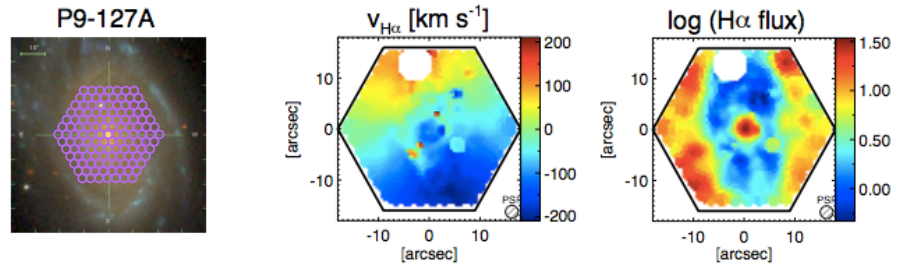
\includegraphics[width=0.95\textwidth]{discussion/manga_data.png}}
\caption[Example MaNGA fibre bundle on a target galaxy with example emission data]{Example fibre bundle placed over a MaNGA target galaxy (left) and corresponding preliminary survey data showing the mapped velocity (middle) and flux (right) of $H\alpha$ gas emission as measured across the galaxy in each fibre. Such measurements can be utilised to calculate the star formation rate across the structure of a galaxy. Adapted from \cite{bundy15} Figure 14.}
\label{fig:manga}
\end{figure}

In Chapter \ref{chap:agn} I discussed how the current SDSS data (both photometric and spectroscopic) cannot determine whether the AGN is the cause or the consequence of the quenching seen across the \textsc{agn-host} population in Figures \ref{time} \& \ref{rate}. Using data from the MaNGA IFU survey \citep{bundy15} I hope to determine whether feedback from the AGN is truly the cause of this quenching. MaNGA is a multi-object IFU survey which by the end of $2020$ will provide IFU spectroscopy for $\sim10,000$ galaxies with a maximum bundle of 127 fibres per galaxy (see Figure~\ref{fig:manga}). Spectral coverage will be continuous from $3,600\rm{\AA}$ to $10,300\rm{\AA}$ out to $1.5~R_e$ for the majority of targets. Although this wavelength range does not encompass the NUV wavelength of $\sim2,300\rm{\AA}$ many spectral indicators of star formation, metallicity and age are all well within this range. This will allow me to modify \starpy\ so that spectral star formation indicators \citep[such as $H\alpha$;][]{kennicutt94} can be used as inputs to break the degeneracy inherent in the photometric colours (see Figure~\ref{pred}). The IFU data will also allow me to remove the contribution of an of any unobscured AGN in the central region of a galaxy. 

Along with these improvements to \starpy, this acquisition of many spectra across the face of a galaxy will allow me to map the inferred quenching parameters as a function of radius. Any correlation of the inferred quenching parameters with radius will allow me to determine whether quenching is happening from the outside-in \citep[i.e. due to environmental mechanisms, as in][]{pan15, clarke16, schaefer17} or inside-out, as in work with preliminary MaNGA survey data by \citet{belfiore16} and with CALIFA data by \citet{gonzalez16}. I will investigate how this preference for outside-in or inside-out quenching is correlated with the presence of an AGN and a galaxy's environment. This will not only help to answer the question of \emph{cause} vs. \emph{consequence} but also further constrain the timescales of quenching mechanisms possibly caused by AGN or the environment. 

A large IFU survey such as MaNGA (with up to $\sim10,000$ galaxies with no cuts on colour or morphology; see \citealt{bundy15}) will also make possible the comparison of large populations of fast and slow rotators. This would aid in the understanding of the different quenching timescales of gas-rich and dry major mergers. I would also like to consider how this kinematic morphological classification of early-type galaxies is linked with the rare PSB phase discussed in Section~\ref{sec:bigpic}. However, considering that $<1\%$ of galaxies are thought to be in this phase at any one time \citep{Wong12, wild16}, within the MaNGA survey only $\lesssim100$ PSB galaxies are expected to be identified. MaNGA is currently the largest IFU survey planned, therefore to investigate the link between PSBs and fast rotators with robust statistics, an IFU survey with $\sim 1$ million target galaxies will be required. 

There is therefore still lots of work that can be done with \starpy. Investigating all of the ideas proposed in this Chapter will most likely take years to complete. However, what I have established in this thesis is a foundation of results which can be built upon with the new influx of large IFU survey data. I have found that the green valley is a transition population between the blue cloud and red sequence, with the rate of transition dependent on morphology. Another key result is the detection of rapid, recent quenching within the \textsc{agn-host} population suggesting tat AGN may be the cause of this quenching via AGN feedback. Not all of the AGN host galaxies however have quenched rapidly, suggesting a slower co-evolution of a galaxy and its black hole. This is supported by the finding that black holes in bulgeless galaxies, with assumed merger free histories, are more massive than predicted by scaling relations between black hole and bulge mass. Along with AGN feedback as a mechanism for quenching, I have found evidence for mergers, environmentally driven quenching mechanisms, mass quenching and morphology quenching all occurring in the group environment, often acting in concert with each other to both achieve and ensure quiescence for a galaxy. 

\section{And one more thought for the road...}\label{sec:hst}

In Chapter~\ref{chap:agn}, I discussed how accurate fits to the bulge-to-total ratio could not be made for galaxies of the \textsc{bulgeless} sample hosting AGN due to the resolution of ground based SDSS imaging. This led to the derivation of upper limits on the bulge masses of this sample. The Hubble Space Telescope (HST) however, provides (i) an extremely stable and well understood point spread function, enabling reliable separation of the AGN from the host galaxy, and (ii) high spatial resolution which is needed to distinguish between classical, merger driven bulges and pseudo bulges grown by secular processes. Observations with the HST of the galaxies in the \textsc{bulgeless} sample will enable extremely robust measures of bulge-to-total ratios for each host galaxy and allow the identification of truly secular systems with growing black holes. Such measurements will also allow the dominance of merger driven (building classical bulges) and merger free (growing pseudo-bulges or retaining a pure disc) co-evolutionary histories to be determined. 

\begin{figure*}
\centering{
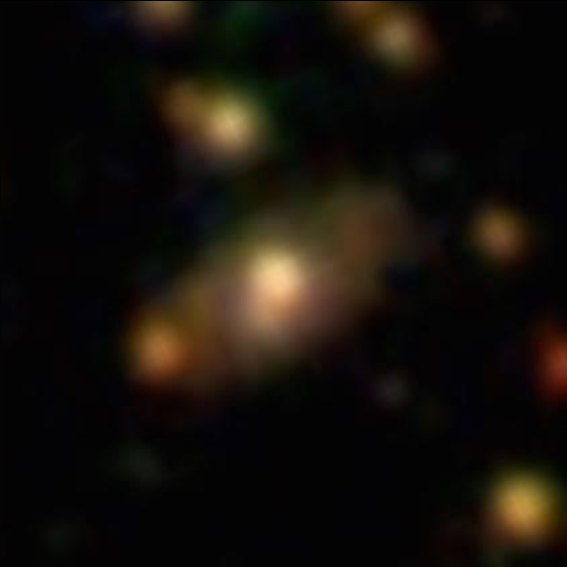
\includegraphics[width=0.49\textwidth]{discussion/sdss_data.png}
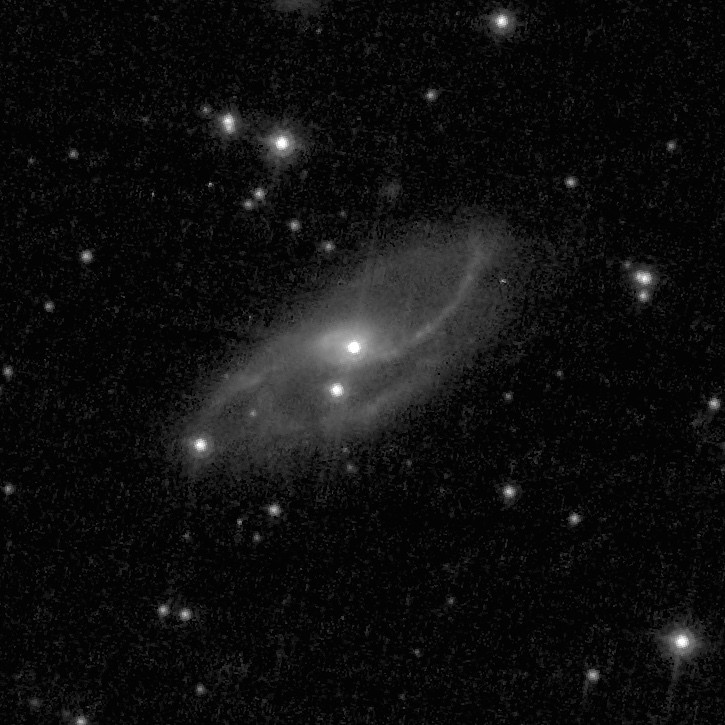
\includegraphics[width=0.49\textwidth]{discussion/hst_data.jpg}}
\caption[Example HST image data in comparison to SDSS]{Example SDSS urgiz image (left) for J$192250.74$-$055259.15$, part of the \textsc{bulgeless} sample, described in Section~\ref{sec:selectAGN}, in comparison to space based imaging from the HST (right). The higher resolution HST image reveals finer structure than the SDSS image, including spiral arms, a ring and a possible bar along with the true disc dominated nature of the galaxy.}
\label{fig:hstdata}
\end{figure*}


We received image data from the HST Advanced Camera for Surveys Wide Field Channel (Proposal ID: 14606, Cycle 24) of the galaxy J$192250.74$-$055259.15$ from the \textsc{bulgeless} sample on October 26th 2016, on which date I was writing Section~\ref{sec:intbulgeless} of this thesis. Figure~\ref{fig:hstdata} demonstrates the difference in resolution provided by the HST with this first image received (right), in comparison with the ground based SDSS ugriz image (left; also shown in Figure~\ref{fig:INTimages}). This galaxy has an estimated black hole mass of $M_{\rm{BH}} = 10^{7.4\pm0.1}~M_{\odot}$ but a bulge-to-total ratio could not be derived from the SDSS image. The HST image will allow for an accurate derivation of the bulge mass of this galaxy, allowing for a more concrete conclusion to be drawn on the controversial issue of secularly driven galaxy-black hole co-evolution. 

